
Selecting the most suitable model was based on inference speed and the model's accuracy in evaluating objects. All experiments were carried out on a Jetson AGX Xavier 32\,GB unit. The model-evaluation experiments were carried out under ideal conditions, which excluded all possible factors that could introduce deviations in the test results of the evaluated model.

These experiments analyse only the neural-network model's processing capability, isolated from the rest of the system (cameras, preprocessing of the frames coming from them, and presentation/transmission of the detected-object information from the frames to other systems), in order to obtain the most optimal and bias-free result regarding model performance and hardware utilisation.

\section{Conducting the experiments}\label{conducting-the-experiments}

The experimental environment conforms to the following conditions:

\begin{enumerate}
\def\labelenumi{\arabic{enumi}.}
\item
  The frames used for inference are specifically selected, standardised, and prepared before the test begins -- i.e., scaled to the size required for the neural-network input and preprocessed. This excludes any additional work or load on the GPU and CPU that would negatively affect the neural network's operation, and allows all the tested models to be evaluated equally on a common dataset.
\item
  Before each test run, the tested models have undergone a hardware warm-up phase -- i.e., have been fully read into the GPU memory of the machine and have run 50 calibration inference iterations using the previously mentioned prepared test frames. This creates an environment in which all models are equally prepared and ready to operate at their maximum capability.
\item
  The number of test runs is 1000, during which the inference speed and detection accuracy on the prepared frames are measured.
\item
  Detection accuracy is evaluated using the following formula:
\end{enumerate}

\begin{quote}
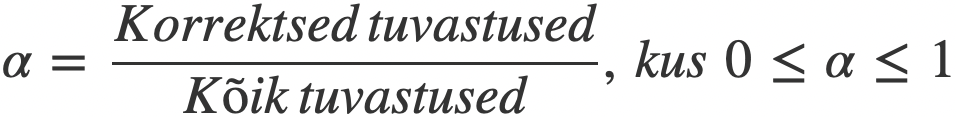
\includegraphics[width=3.18442in,height=0.37002in]{media/image23.png}

The closer the result is to one, the more accurate the model and the more capable it is of detecting objects.
\end{quote}

\begin{enumerate}
\def\labelenumi{\arabic{enumi}.}
\setcounter{enumi}{4}
\tightlist
\item
  The model's speed is evaluated by the time taken for inference in milliseconds (shown in the charts as the number of frames processed in one second).
\end{enumerate}

Jetson AGX Xavier software configuration:

\begin{itemize}
\item
  JetPack 5.0.2
\item
  Ubuntu 20.04.5
\item
  kernel 5.10.104-tegra
\item
  L4T 35.1.0
\item
  Python 3.8.10
\item
  torch 1.12.0
\item
  torchvision 0.13.0
\item
  cv2 4.5.0
\item
  TensorRT 8.4.1.5
\item
  CUDA 11.4
\end{itemize}

\section{Analysis of results}\label{analysis-of-results}

The experiments were run in two configurations: with one frame and with three frames processed in parallel, since in the production environment the neural network processes information from three frames. The \emph{mean Average Precision} parameter shown in the charts (in yellow) expresses the model's mean total accuracy across all classes; it is derived from experiments carried out on classes selected from the COCO 2017 validation dataset, with an equal number of test samples chosen from all classes \cite{ref64}. The \emph{accuracy} parameter (in red) was obtained on a separately created dataset containing only vessels. Results are shown in ascending order of model size (number of parameters) -- the smallest model on the left, the largest on the right -- to provide an intuitive overview of all parameters.

The accuracy fluctuations seen in the charts for models with larger inputs (see Figures~\ref{fig:image25} and~\ref{fig:image27}) are due to the fact that the scaling layers of the ``6''-suffixed models were designed for larger input resolutions, while the layers of the other models were designed for smaller input resolutions \cite{ref65}. The latter therefore exhibit lower accuracy at this resolution.

The speed difference between optimised and unoptimised models is at least twofold; the largest speed difference is 4.28$\times$, for the yolov5l6 pair (see Figure~\ref{fig:image26}). The accuracy difference between optimised and unoptimised models is minimal ($1.7 \cdot 10^{-3}$), i.e.\ optimisation did not significantly affect accuracy. As a result, the accuracy values initially shown on the chart overlapped, so their averaged values are displayed instead.

\begin{figure}[H]
\centering
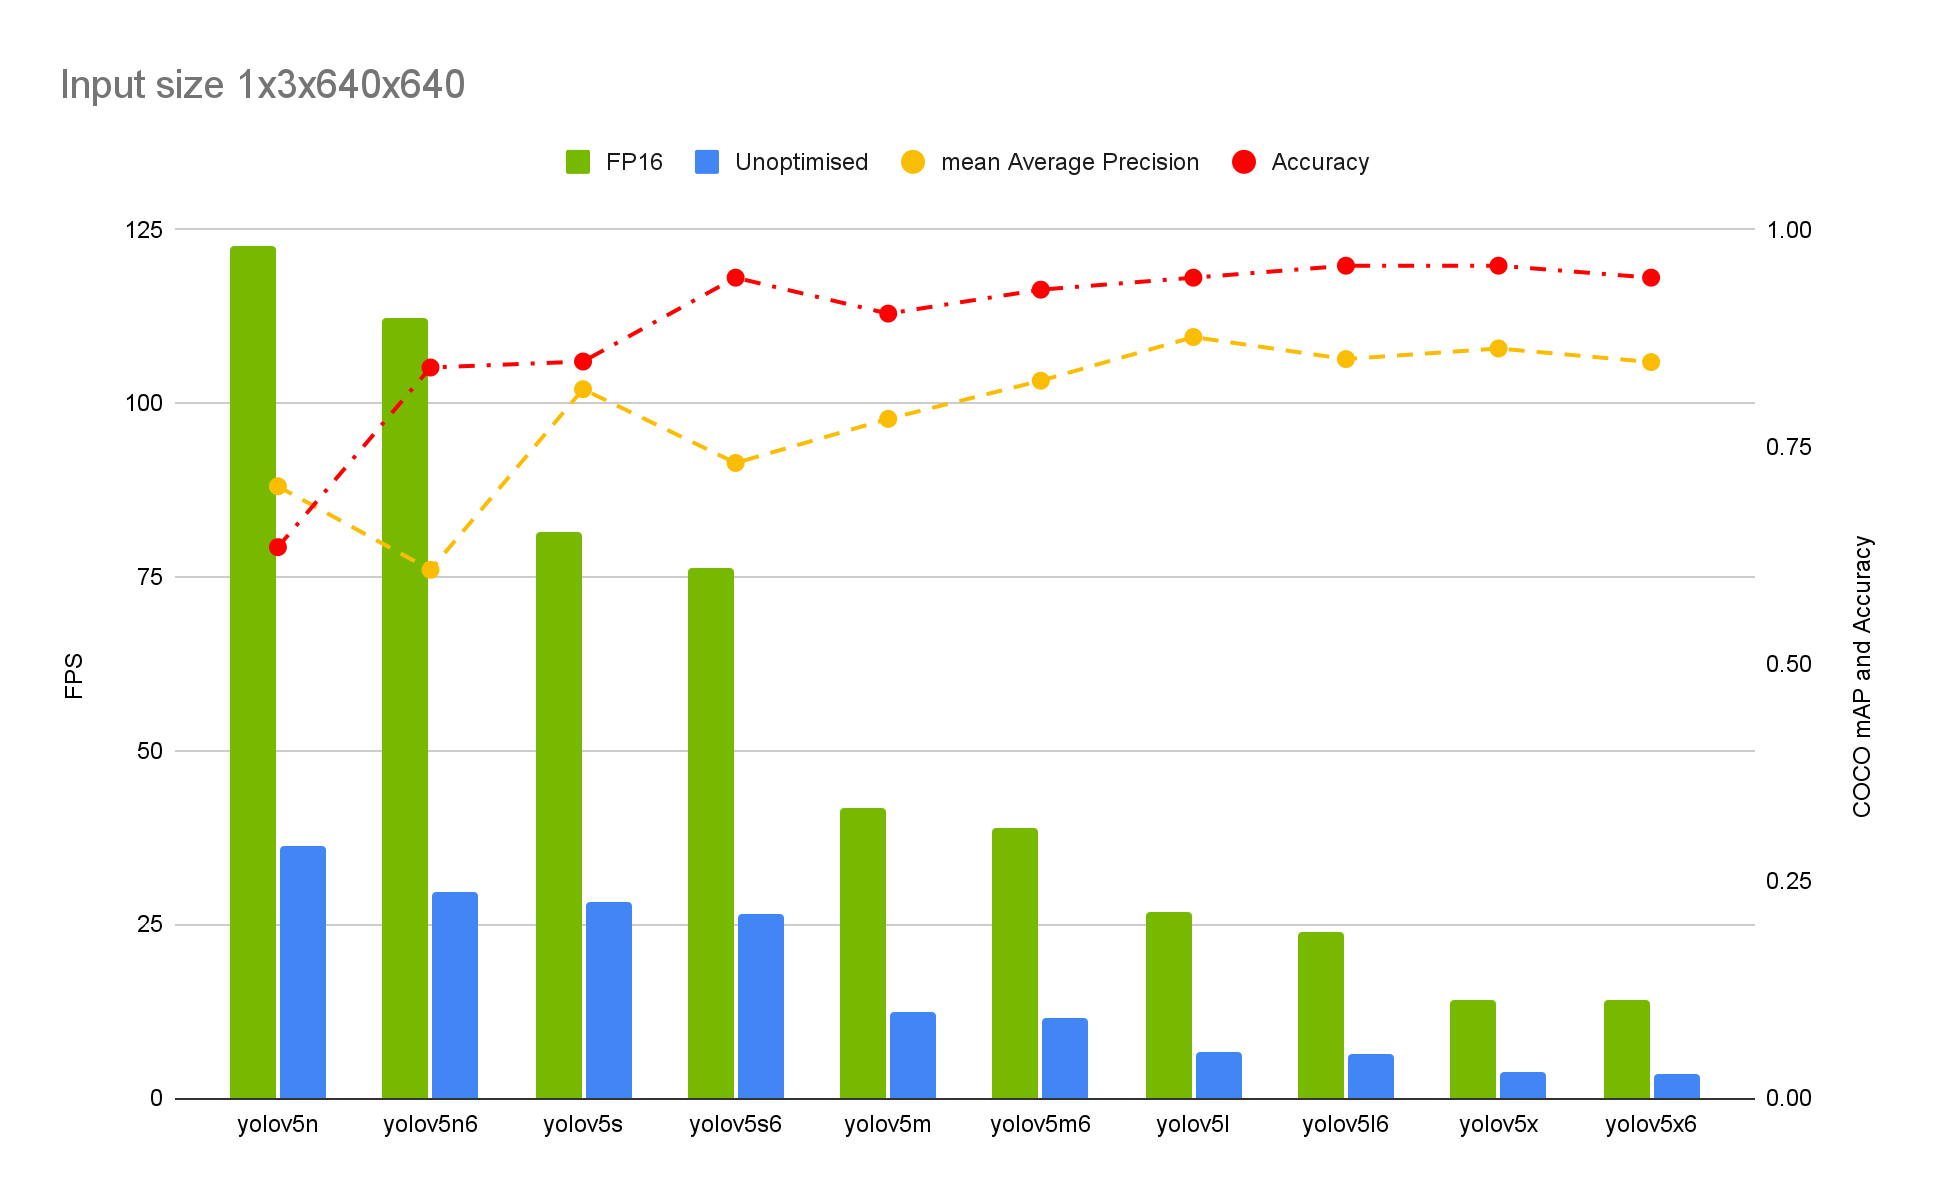
\includegraphics[width=6.10174in,height=3.77778in,alt={Input size 1x3x640x640}]{media/image24.png}
\caption{Model performance with a single 640$\times$640-pixel frame input}\label{fig:image24}
\end{figure}

The speed difference between the fastest and slowest optimised model is 108 frames per second, with the best speed-up being fourfold. The mean optimised speed difference is 3.5$\times$. Model accuracy grows up to the YOLOv5l model and there is no significant accuracy gain beyond it; from that model onward the speed-to-accuracy ratio decreases.

\begin{figure}[H]
\centering
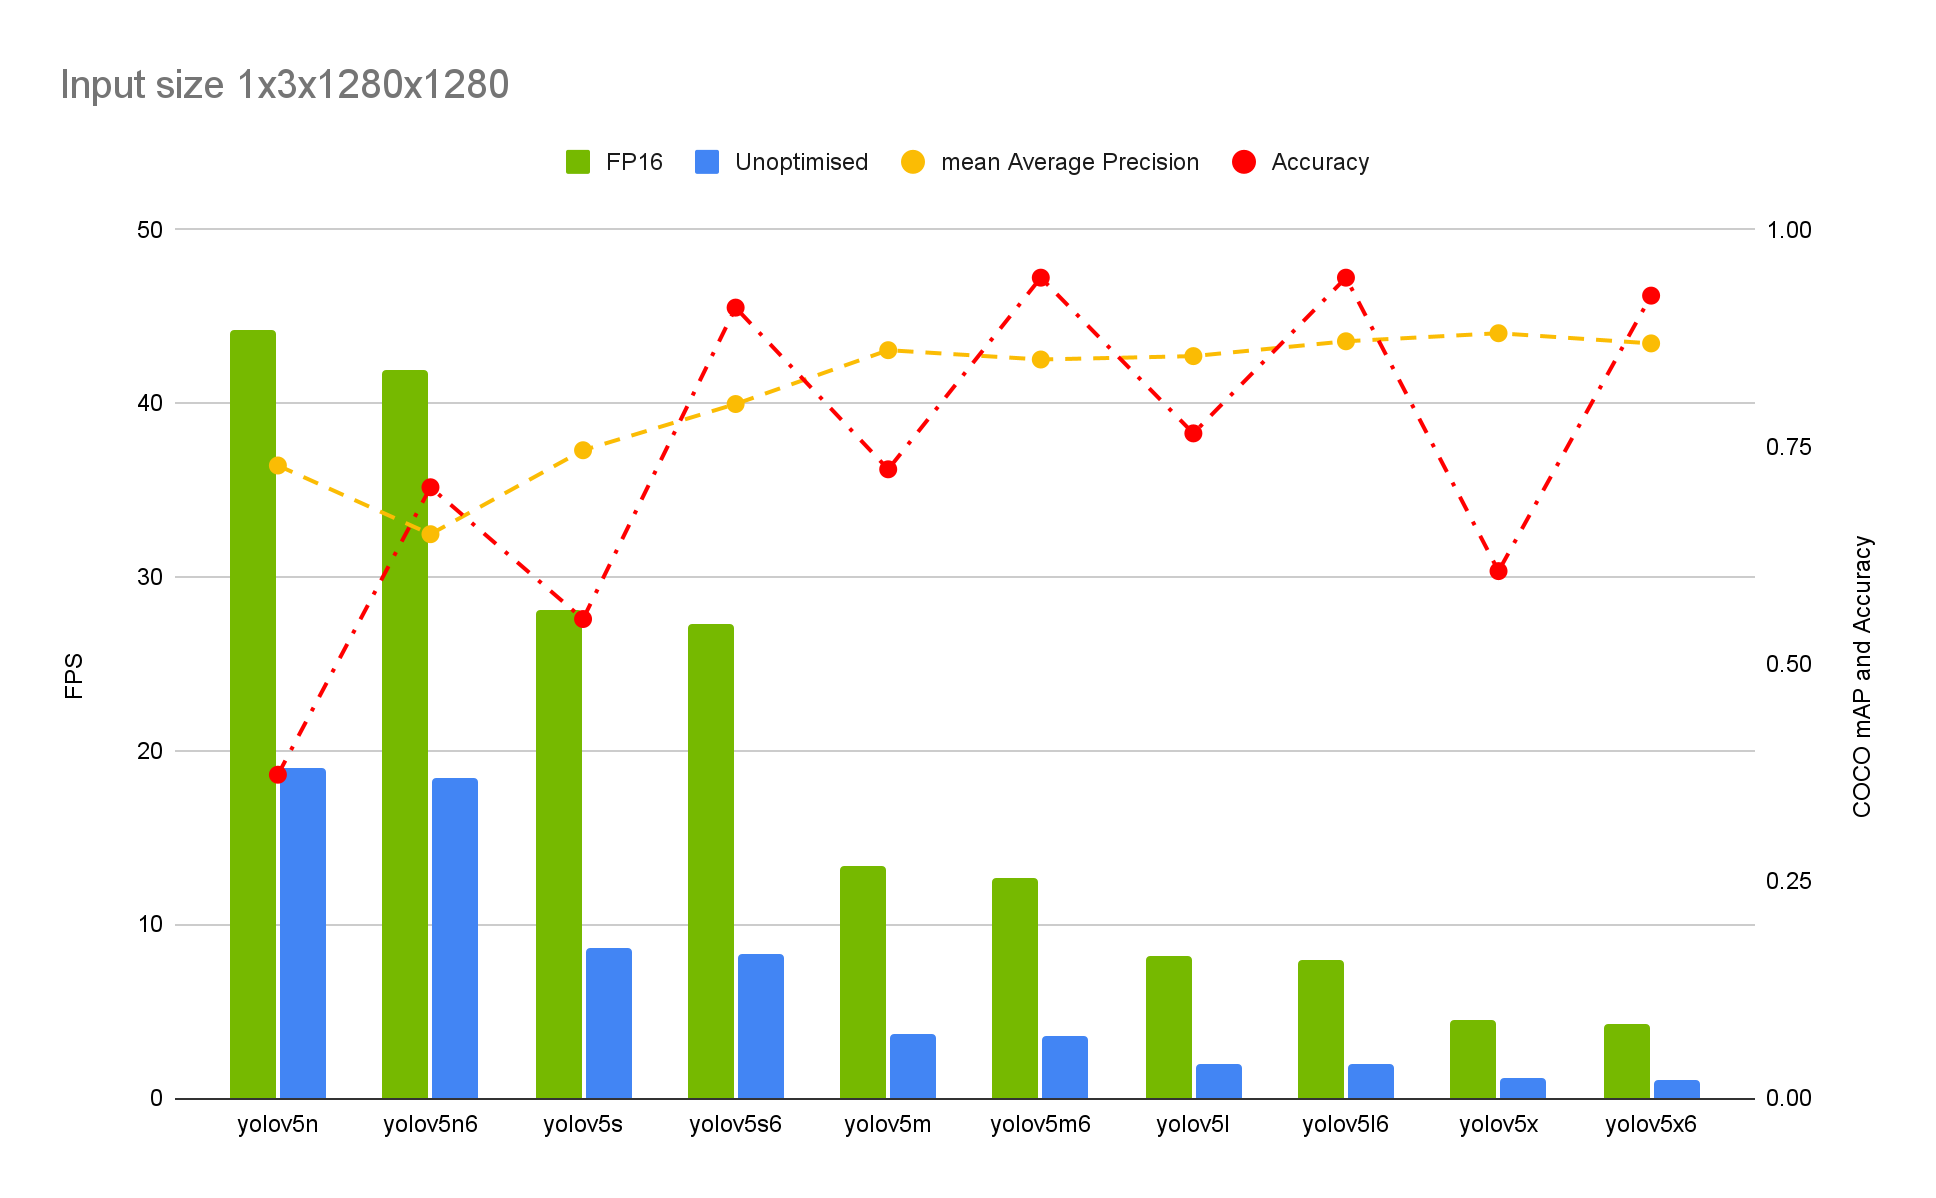
\includegraphics[width=6.10174in,height=3.77778in,alt={Input size 1x3x1280x1280}]{media/image25.png}
\caption{Model performance with a single 1280$\times$1280-pixel frame input}\label{fig:image25}
\end{figure}

The speed difference between the fastest and slowest optimised model is 40 frames per second, with the best speed-up of 4.1$\times$. The mean optimised speed difference is 3.5$\times$. Model accuracy grows up to the YOLOv5m model and there is no significant gain beyond it; from that model onward the speed-to-accuracy ratio decreases.

The mean speed difference between the single-input 640$\times$640 and 1280$\times$1280 models is 36 frames per second.

\begin{figure}[H]
\centering
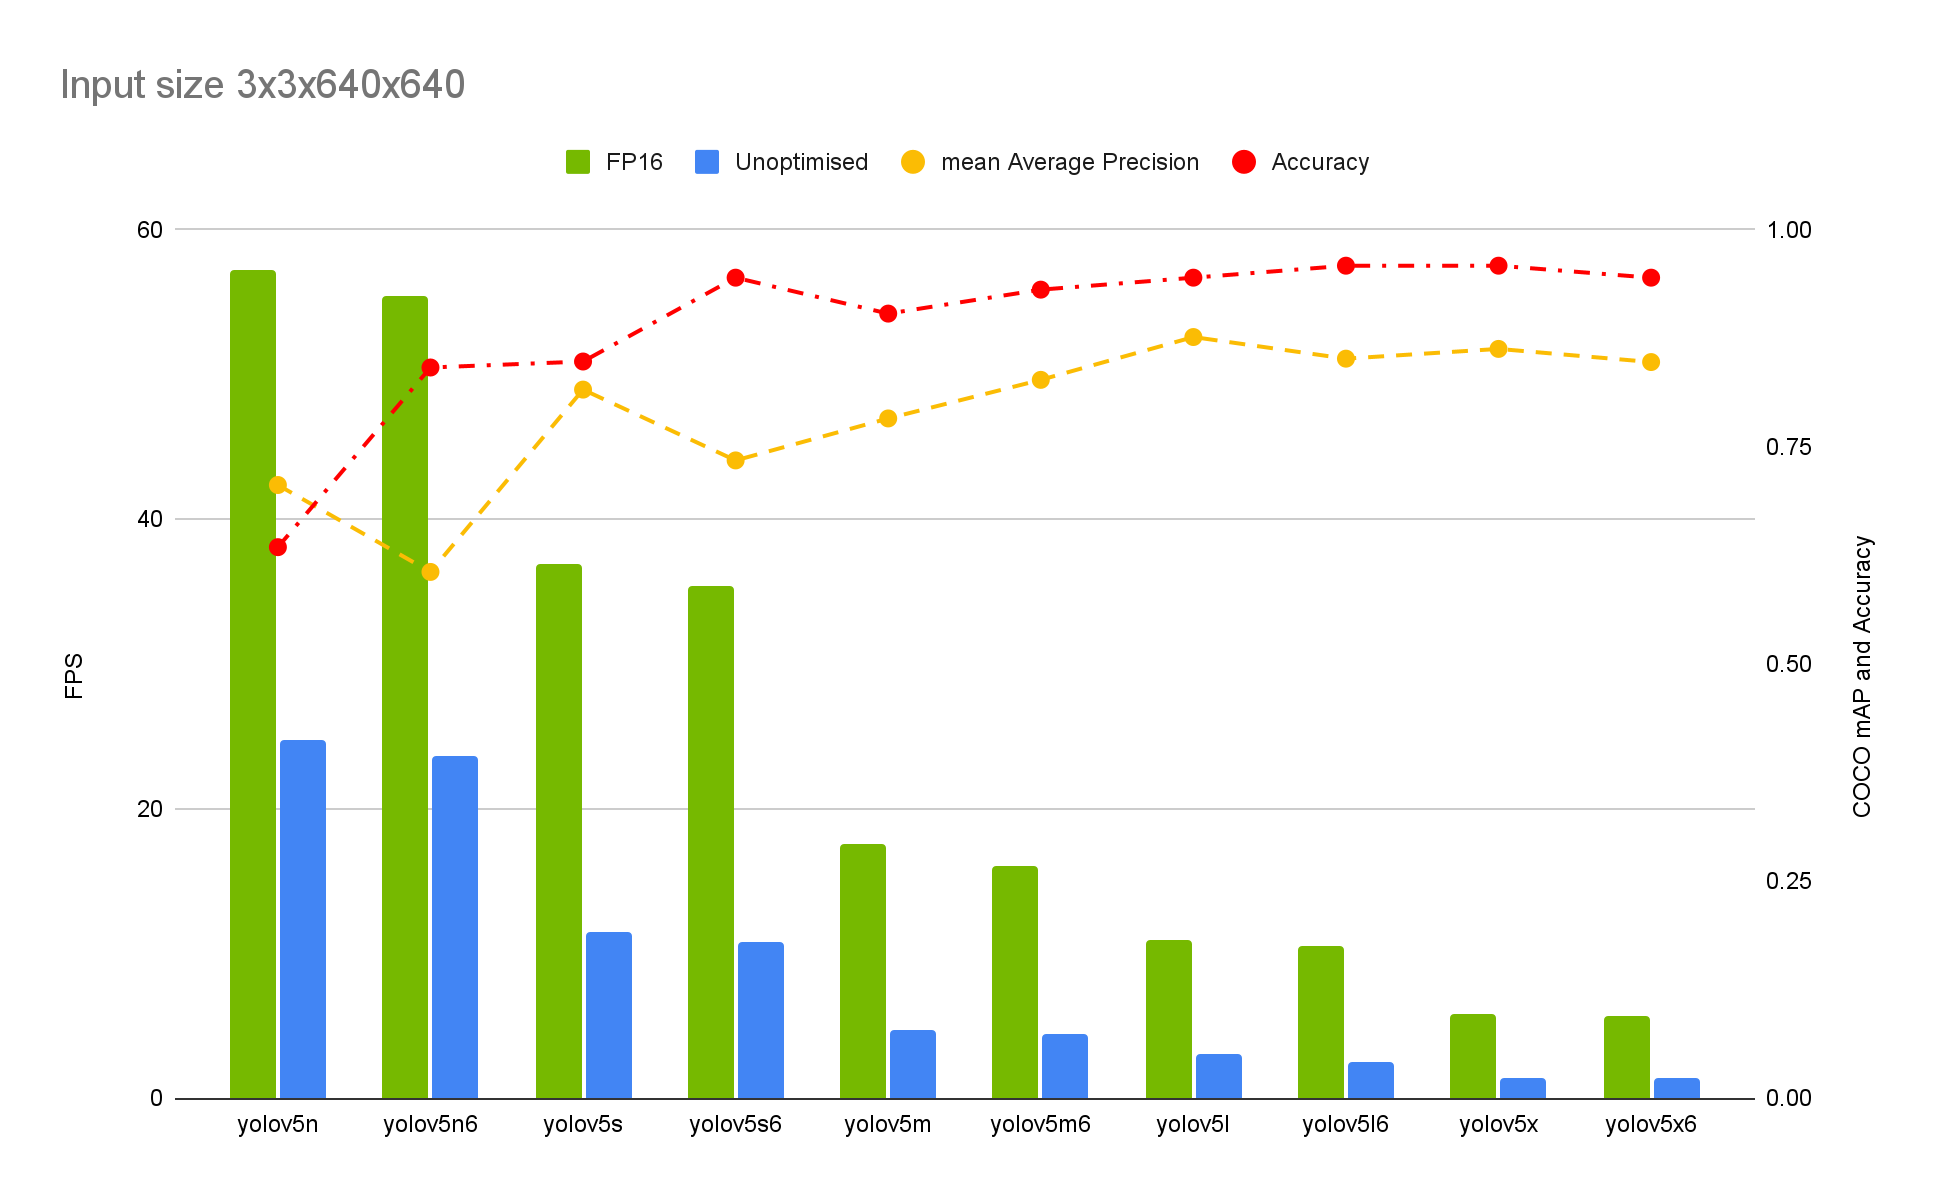
\includegraphics[width=6.10174in,height=3.77778in,alt={Input size 3x3x640x640}]{media/image26.png}
\caption{Model performance with three 640$\times$640-pixel frame inputs in parallel}\label{fig:image26}
\end{figure}

The speed difference between the fastest and slowest optimised model is 52 frames per second, with the best speed-up of 4.3$\times$. The mean optimised speed difference is 3.4$\times$. Model accuracy grows up to the YOLOv5l model and there is no significant gain beyond it; from that model onward the speed-to-accuracy ratio decreases.

The three-input 640$\times$640 models are on average 1.4$\times$ faster than the single-input models at the same resolution.

\begin{figure}
\centering
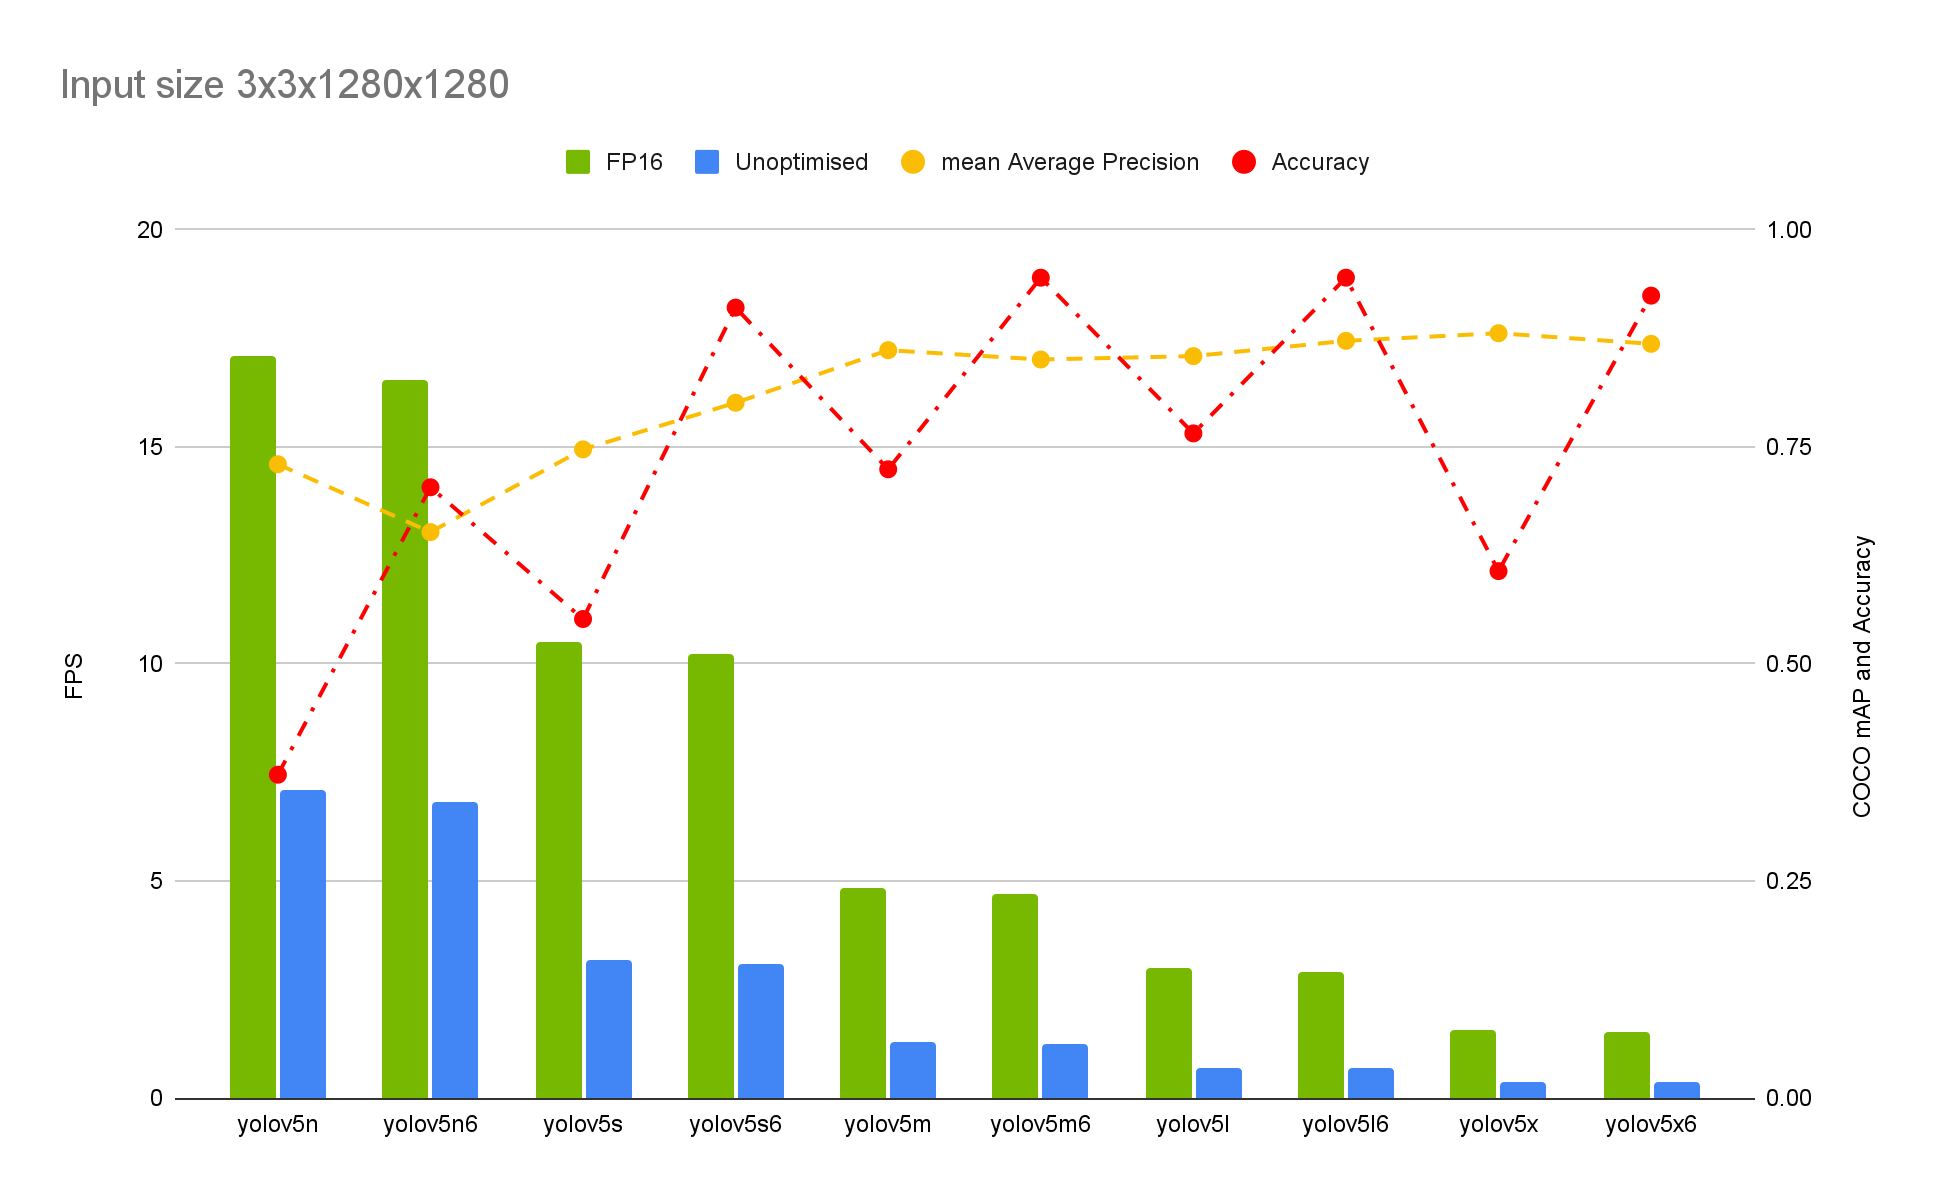
\includegraphics[width=6.10174in,height=3.77778in,alt={Input size 3x3x1280x1280}]{media/image27.png}
\caption{Model performance with three 1280$\times$1280-pixel frame inputs in parallel}\label{fig:image27}
\end{figure}

The speed difference between the fastest and slowest optimised model is 16 frames per second, with the best speed-up of 4.2$\times$. The mean optimised model speed difference is 3.5$\times$. Model accuracy grows up to the YOLOv5m model and there is no significant gain beyond it; from that model onward the speed-to-accuracy ratio decreases. In this case the models are 1.1$\times$ faster than the single-input models at the same resolution.

The mean speed difference between the three-input 640$\times$640 and 1280$\times$1280 models is 18 frames per second.

The three-input models are on average 1.2$\times$ faster than the single-input models.
